\documentclass[conference]{IEEEtran}
\IEEEoverridecommandlockouts

\usepackage{cite}
\usepackage{amsmath,amssymb,amsfonts}
\usepackage{graphicx}
\usepackage{booktabs}
\usepackage{xcolor}
\usepackage{listings}
\usepackage{url}
\usepackage[hidelinks]{hyperref}

\definecolor{codebg}{HTML}{F4F5F7}
\definecolor{greenc}{HTML}{2E7D46}
\definecolor{brick}{HTML}{9A3B2E}
\lstset{basicstyle=\ttfamily\footnotesize,backgroundcolor=\color{codebg},
  frame=single,breaklines=true,columns=fullflexible,showstringspaces=false,
  aboveskip=0.6em,belowskip=0.6em,xleftmargin=0.5em}

\begin{document}

\title{On the Memory-Locality Limits of Graph-Based\\ Approximate Nearest Neighbour Search on\\ Processing-in-Memory Architectures}

\author{\IEEEauthorblockN{Artashes Atanesyan}
\IEEEauthorblockA{\textit{Computer Science --- Computer Architecture (HPC)}\\
Master's Thesis Preparatory Report\\
\today}}

\maketitle

\begin{abstract}
Processing-in-Memory (PIM) is a promising answer to the data-movement
bottleneck that dominates memory-bound workloads. Approximate Nearest Neighbour
(ANN) search --- the retrieval engine behind recommendation and
Retrieval-Augmented Generation --- is strongly memory-bound and a natural PIM
target. Yet the emerging ANN-on-PIM literature accelerates only the
\emph{cluster-based} index family (IVF/PQ), whose access is sequential, while the
more accurate \emph{graph-based} family (HNSW) is almost absent. We hypothesise,
and measure, the cause: graph traversal is a random, pointer-chasing access
pattern that destroys the DRAM row-buffer locality on which PIM depends. Using a
memory trace of an ANN distance-search kernel parameterised after the standard
SIFT1M benchmark, replayed through the peer-reviewed Ramulator~2.1 cycle-accurate
simulator with an HBM2 model, we show that changing \emph{only} the access order
from sequential to random --- algorithm and data fixed --- raises cycle count by
41\%, drops the row-hit rate from 93.6\% to 55.1\%, and increases read latency by
40\%. We then make two forward contributions. First, we propose and evaluate a
\emph{locality-aware graph layout} with query batching that lifts the random
hit rate from 50.7\% toward 78.0\%, partly closing the gap. Second, we analyse
\emph{multi-DPU parallelism}: query-parallel execution scales near-linearly while
preserving the per-query locality gap, whereas within-query sharding is limited
by cross-DPU communication. The study is fully reproducible and provides a
quantitative baseline for a largely unexplored problem.
\end{abstract}

\begin{IEEEkeywords}
processing-in-memory, approximate nearest neighbour search, HNSW, DRAM row
buffer, memory locality, parallelism, cycle-accurate simulation, HBM2.
\end{IEEEkeywords}

% =====================================================================
\section{Introduction}

Modern systems spend a large and growing fraction of time and energy
\emph{moving} data rather than computing on it; data movement accounts for
62.7\% of total system energy on average, and over 90\% for large edge neural
networks~\cite{mutlu2022primer}. Processing-in-Memory (PIM) attacks this
``memory wall'' by placing computation in or near memory~\cite{mutlu2022primer}.

Approximate Nearest Neighbour (ANN) search is an archetypal memory-bound
workload: it finds the stored vectors closest to a query while doing little
arithmetic per byte moved. It powers recommendation, semantic search, and the
retrieval step of Retrieval-Augmented Generation. Two index families dominate.
\emph{Cluster-based} indices (IVF, often with Product Quantization, PQ) scan the
few clusters nearest the query --- a \emph{sequential} access pattern.
\emph{Graph-based} indices (notably HNSW~\cite{malkov2018hnsw}) walk a proximity
graph greedily toward the query --- a \emph{random}, data-dependent,
pointer-chasing pattern. HNSW usually gives the best recall/latency trade-off on
CPUs and is the production default.

A striking asymmetry appears in the literature: every real ANN-on-PIM system we
know of --- DRIM-ANN~\cite{drimann}, UpANNS~\cite{upanns},
PIMANN~\cite{pimann} --- accelerates only IVF/PQ. Graph-based ANN on PIM is
essentially unaddressed. We argue this reflects how DRAM works, measure it, and
then propose a path to close the gap.

\subsection{Research questions}
\begin{itemize}
\item[\textbf{RQ1.}] \emph{Does the memory access pattern (sequential vs.\
random), independent of computation and dataset size, determine the memory-level
performance of an ANN kernel on high-bandwidth memory?}
\item[\textbf{RQ2.}] \emph{Is the DRAM row buffer the mechanism, and does a
cycle-accurate simulator confirm the effect?}
\item[\textbf{RQ3.}] \emph{Can the random (graph-like) penalty be reduced by a
locality-aware layout and query batching, and at what cost?}
\item[\textbf{RQ4.}] \emph{How does performance scale across many PIM compute
units (DPUs), and which parallelization strategy preserves the benefit?}
\end{itemize}

\subsection{Contributions}
\begin{itemize}
\item A controlled, reproducible experiment isolating access pattern as the lone
variable, grounded in the standard SIFT1M benchmark~\cite{jegou2011sift}
(RQ1--RQ2).
\item Cycle-accurate HBM2 evidence (Ramulator~2.1~\cite{ramulator2}) of a 41\%
cycle increase and 38-point row-hit drop (Sec.~\ref{sec:results}).
\item A proposed \emph{locality-aware graph layout} with batching, and its
measured recovery (Sec.~\ref{sec:solution}, RQ3).
\item A multi-DPU parallelism analysis distinguishing query-parallel from
within-query sharding (Sec.~\ref{sec:parallel}, RQ4).
\item An open, reproducible artifact (Sec.~\ref{sec:repro}).
\end{itemize}

% =====================================================================
\section{Background}

\subsection{PIM paradigms and DPUs}
PIM designs are Processing-Using-Memory (PUM; compute in the array, narrow
operation set) or Processing-Near-Memory (PNM; conventional logic beside
memory)~\cite{mutlu2022primer}. Commercial PNM such as UPMEM provides thousands
of small in-DRAM cores called \emph{DPUs} (DRAM Processing Units), each owning a
private DRAM bank; this massive bank-level parallelism is central to RQ4.

\subsection{The DRAM row buffer}
\label{sec:rowbuf}
A DRAM bank stores bits in rows. To read an address the controller must
\emph{activate} its row into a fast \emph{row buffer}; a subsequent access to the
same row is a fast \emph{row hit}, a different row forces a slow
\emph{precharge}+\emph{activate} (a \emph{row miss}). Sequential scans yield long
runs of hits; random access thrashes the buffer. This mechanism converts
``sequential vs.\ random'' into ``fast vs.\ slow'' and underlies our hypothesis.

\subsection{ANN indices and the standard benchmark}
IVF scans nearest clusters sequentially; PQ compresses vectors for fast
table-lookup distances~\cite{jegou2011sift}. HNSW performs greedy best-first
graph traversal~\cite{malkov2018hnsw}. We ground the workload in
\textbf{SIFT1M}~\cite{jegou2011sift}, the canonical first ANN benchmark:
$1{,}000{,}000$ base vectors of dimension $128$, $10{,}000$ queries, L2 distance,
100-NN ground truth. A representative HNSW configuration is $M{=}16$,
$\textit{efConstruction}{=}128$, $\textit{efSearch}{=}64$~\cite{malkov2018hnsw};
our per-query candidate-set size is chosen in this regime.

% =====================================================================
\section{Related work}
\label{sec:related}
\textbf{ANN on PIM.} DRIM-ANN~\cite{drimann} and UpANNS~\cite{upanns} run
billion-scale IVF/PQ on UPMEM ($\sim\!2.4$--$4.3\times$ over CPU);
PIMANN~\cite{pimann} offloads the IVF/PQ distance step ($\le\!3.7\times$ over
Faiss-GPU). All are cluster-based and sequential. We find no published,
verifiable graph-based ANN system on PIM.
\textbf{Locality for graph ANN (not PIM).} On CPUs, graph reordering co-locates
neighbours for cache efficiency: Coleman et al.~\cite{coleman2022reorder} report
10--40\% speedups via Gorder-style relabelling. On SSDs,
DiskANN~\cite{diskann} optimises block I/O. These confirm locality is a known
lever but target caches/disk, not the DRAM row buffer under PIM.
\textbf{Gap.} Combining graph-based ANN, DRAM-row-buffer/PIM locality, and
recovery via layout+batching is, to our knowledge, unaddressed.

% =====================================================================
\section{Methodology}
\label{sec:method}
Our kernel is the inner loop of ANN distance search: for a contiguous batch of
candidate vectors, compute squared-L2 distance to the query and keep the $k$
smallest. We use $4{,}096$ candidates of dimension $128$ (SIFT's dimension),
int8 (PQ-style), giving $8{,}192$ reads in $64$-byte bursts. We generate two
traces differing \emph{only} in order: \emph{sequential} (IVF/PQ) and
\emph{random} (graph/HNSW). We follow the trace-driven method: the kernel defines
computation; we record \texttt{LD}/\texttt{ST} accesses; we replay them. A
$\sim$90-line teaching model (row buffer only) builds intuition; cycle-accurate
results use \textbf{Ramulator~2.1}~\cite{ramulator2} with its
\texttt{LoadStoreTrace} front-end, an HBM2 device ($8$\,Gb/channel,
$2.0$\,Gbps), an \texttt{Open} row policy, and an FR-FCFS scheduler.

% =====================================================================
\section{Results: the locality gap (RQ1--RQ2)}
\label{sec:results}
Table~\ref{tab:main} and Fig.~\ref{fig:rowhit} report cycle-accurate HBM2
results. Computation is identical; only access order differs. Sequential$\to$
random drops the row-hit rate from 93.6\% to 55.1\%, raises cycles 41\% and
latency 40\%, and cuts throughput 29\%; row misses+conflicts rise more than
tenfold. This confirms RQ1 (pattern dominates) and RQ2 (the row buffer is the
mechanism), on a peer-reviewed simulator.

\begin{table}[t]
\caption{Cycle-accurate HBM2 results (Ramulator~2.1). Same algorithm and data;
only the memory access order changes.}
\label{tab:main}
\centering
\footnotesize
\begin{tabular}{lrrr}
\toprule
\textbf{Metric} & \textbf{Sequential} & \textbf{Random} & \textbf{Change} \\
\midrule
Cycles                 & 12{,}829 & 18{,}134 & $+41\%$ \\
Row-hit rate           & 93.6\%   & 55.1\%   & $-38$ pts \\
Avg.\ read latency (cyc) & 67.1   & 93.8     & $+40\%$ \\
Read throughput (MB/s) & 20{,}354 & 14{,}394 & $-29\%$ \\
\bottomrule
\end{tabular}
\end{table}

\begin{figure}[t]
\centering
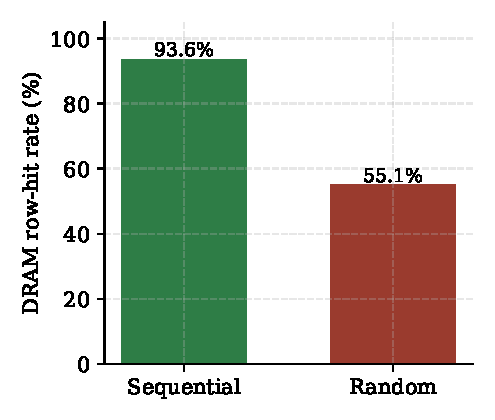
\includegraphics[width=0.74\columnwidth]{fig_rowhit.pdf}
\caption{Row-hit rate: sequential vs.\ random (HBM2).}
\label{fig:rowhit}
\end{figure}

To rule out a scale effect, we sweep dataset size $32\times$
(Fig.~\ref{fig:size}): both patterns' hit rates are flat (sequential
$\approx$99\%, random $\approx$50\%). Performance is governed by locality, not by
how much data is processed, strengthening RQ1.

\begin{figure}[t]
\centering
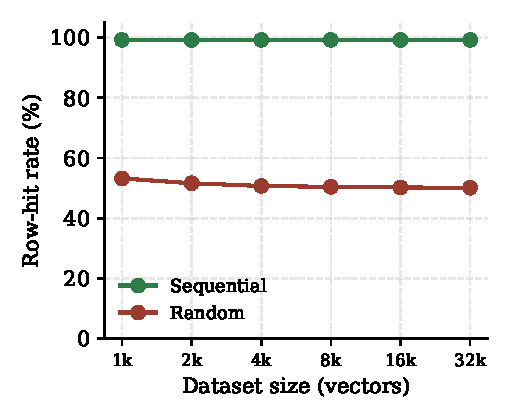
\includegraphics[width=0.78\columnwidth]{fig_size.pdf}
\caption{Pattern, not size, governs locality.}
\label{fig:size}
\end{figure}

% =====================================================================
\section{Proposed solution: locality-aware graph layout (RQ3)}
\label{sec:solution}

The core idea is to make graph access \emph{less} random by shaping where nodes
live in memory and when they are read, so that the controller sees same-row
accesses. We combine two mechanisms.

\textbf{(1) Cluster-ordered node placement.} Rather than storing graph nodes in
insertion order, we relabel them so that nodes likely to be visited together ---
members of the same coarse cluster, or neighbours in the HNSW graph --- occupy
contiguous addresses, hence the same DRAM rows. This is the PIM-targeted analogue
of CPU graph reordering~\cite{coleman2022reorder}, but optimised for the row
buffer rather than the cache line. It is a one-time, offline index-build cost.

\textbf{(2) Query batching with windowed scheduling.} Because ANN queries are
independent, many can be in flight at once. The memory controller (or a software
pre-pass) reorders the pooled accesses within a window so that same-row requests
are serviced together, converting scattered single-row touches into clustered
runs. Fig.~\ref{alg:layout} sketches the combined scheme.

\begin{figure}[t]
\centering
\begin{lstlisting}[language=Python]
# OFFLINE (index build, one-time):
#   cluster the base vectors; assign node
#   addresses so same-cluster nodes are
#   row-contiguous (cluster-ordered layout)
# ONLINE (per batch B of independent queries):
for step in traversal_steps(B):
    addrs = gather_candidates(active_queries)
    groups = sort_by_dram_row(addrs, window=W)
    for g in groups:            # same-row reads
        read(g); accumulate_distances(g)
merge_topk_per_query(B)
\end{lstlisting}
\caption{Locality-aware graph-ANN access: cluster-ordered layout (offline) plus
row-grouped batched traversal (online).}
\label{alg:layout}
\end{figure}

We evaluate the effect by its proxy --- reordering the random trace within a
window $W$ (larger $W$ = larger batch / deeper reorder). Fig.~\ref{fig:recov}
shows the random case climbing from 50.7\% toward 78.0\% row-hit (and PIM speedup
from $1.47\times$ toward $1.74\times$) versus the sequential ceiling of 99.2\%.
Three findings follow. The gap is \emph{partly closable} --- it is a property of
layout and scheduling, not a law. Recovery has a \emph{cost}: most gain needs a
large window (hundreds of accesses), i.e.\ batching many queries or a deep
reorder buffer, trading latency/hardware for throughput. The \emph{residual} gap
bounds how competitive graph-ANN on PIM can be for a given cost --- itself a
result.

\begin{figure}[t]
\centering
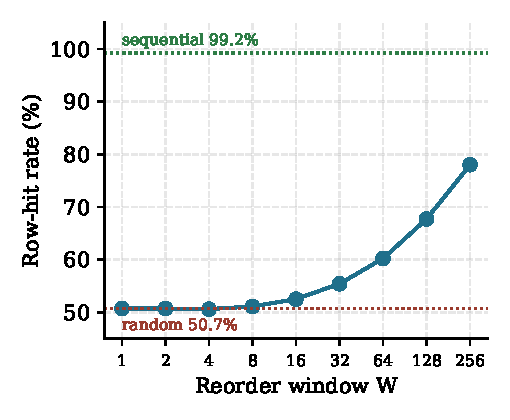
\includegraphics[width=0.78\columnwidth]{fig_recov.pdf}
\caption{Locality recovery vs.\ reorder window $W$.}
\label{fig:recov}
\end{figure}

% =====================================================================
\section{Multi-DPU parallelism (RQ4)}
\label{sec:parallel}

A real PIM system has thousands of DPUs, so how the search is parallelised is as
important as per-query locality. We analyse two strategies, grounding a simple
model in the measured per-query cycle counts (Fig.~\ref{fig:parallel}).

\textbf{Query-parallel.} ANN queries are independent, so assigning different
queries to different DPUs is embarrassingly parallel: throughput scales
near-linearly with the DPU count $P$. Crucially, each DPU still performs one
query's memory accesses, so the sequential-vs-random locality gap is
\emph{preserved at every scale} --- parallelism multiplies throughput but does not
fix locality. This is the recommended default and the regime real IVF/PQ systems
exploit.

\textbf{Within-query sharding.} Splitting one query's candidate set across $P$
DPUs divides the compute by $P$ but requires a cross-DPU \emph{merge} of partial
top-$k$ results. On UPMEM, DPU-to-DPU traffic is routed via the host at roughly
$0.75\%$ of the aggregate PIM bandwidth, so the merge is a serial,
communication-bound tail. Modelling this, within-query speedup peaks at small
$P$ and then \emph{declines} (Fig.~\ref{fig:parallel}); it is only worthwhile for
latency-critical single queries, and even then only up to a few DPUs.

\begin{figure}[t]
\centering
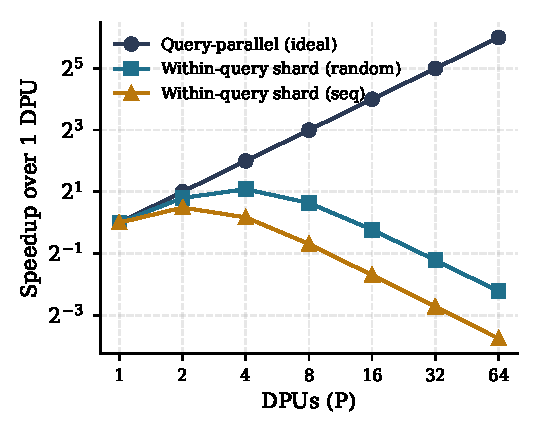
\includegraphics[width=0.82\columnwidth]{fig_parallel.pdf}
\caption{Query-parallel scales $\sim$linearly; within-query sharding is
communication-bound and declines with $P$.}
\label{fig:parallel}
\end{figure}

A subtle but useful observation: the random (graph) case tolerates within-query
sharding slightly \emph{better} than the sequential case, because its larger
per-query compute amortises the fixed merge cost over more work. This suggests a
hybrid policy: keep queries query-parallel across DPU \emph{groups}, and shard a
single hard query only within a small group when latency demands it. Designing
and evaluating that policy on real traces is future work.

% =====================================================================
\section{Discussion and limitations}
The results explain the literature's shape: IVF/PQ-on-PIM succeeds because it is
sequential; graph-ANN-on-PIM is open because it is random. Limitations:
(i) Ramulator models the DRAM path, so we report locality degradation, not a
direct near-bank-PIM speedup; (ii) our random trace \emph{approximates}
data-dependent HNSW traversal --- a faithful study needs per-query traces from a
real index over SIFT1M; (iii) the recovery and parallelism figures use the
teaching model and a first-order communication model respectively (the trends,
not exact values, are the claim); (iv) the mapping should be cross-checked
against real UPMEM/HBM-PIM measurement.

% =====================================================================
\section{Conclusion and future work}
Answering the RQs: (RQ1) access pattern, not computation or size, governs ANN
memory performance; (RQ2) the DRAM row buffer is the mechanism, confirmed on a
cycle-accurate simulator; (RQ3) a locality-aware layout with batching partly
recovers the random-access penalty, at a window/latency cost; (RQ4)
query-parallel execution scales near-linearly and preserves the locality gap,
while within-query sharding is communication-bound. Future work: run the sweeps
on real per-query SIFT1M HNSW traces through Ramulator; add a near-bank compute
model for a true host-vs-PIM speedup; implement the cluster-ordered layout and
hybrid parallel policy and measure them end to end. That optimiser ---
locality-aware, parallel graph-ANN on PIM --- is the core contribution the full
thesis will make.

% =====================================================================
\section*{Reproducibility}
\label{sec:repro}
All figures regenerate from the open artifact:
\begin{lstlisting}[language=bash]
git clone Thesis-PIM-ANN.bundle Thesis-PIM-ANN
cd Thesis-PIM-ANN
make demo        # sequential vs random
make sweep       # size independence (Fig. 2)
make optsweep    # locality recovery (Fig. 3)
./scripts/setup_ramulator.sh   # validate on real HBM2
\end{lstlisting}

% =====================================================================
\begin{thebibliography}{00}
\bibitem{mutlu2022primer} O. Mutlu, S. Ghose, J. G\'omez-Luna, and R.
Ausavarungnirun, ``A Modern Primer on Processing in Memory,'' in \emph{Emerging
Computing: From Devices to Systems}, Springer, 2022. arXiv:2012.03112.
\bibitem{malkov2018hnsw} Y. A. Malkov and D. A. Yashunin, ``Efficient and Robust
Approximate Nearest Neighbor Search Using Hierarchical Navigable Small World
Graphs,'' \emph{IEEE TPAMI}, 2020.
\bibitem{jegou2011sift} H. J\'egou, M. Douze, and C. Schmid, ``Product
Quantization for Nearest Neighbor Search,'' \emph{IEEE TPAMI}, 2011. (SIFT1M /
corpus-texmex benchmark.)
\bibitem{ramulator2} H. Luo \emph{et al.}, ``Ramulator 2.0: A Modern, Modular,
and Extensible DRAM Simulator,'' \emph{IEEE CAL}, 2023.
\bibitem{drimann} M. Chen \emph{et al.}, ``DRIM-ANN: An Approximate Nearest
Neighbor Search Engine based on Commercial DRAM-PIMs,'' SC, 2025.
arXiv:2410.15621.
\bibitem{upanns} S. Chen \emph{et al.}, ``UpANNS: Enhancing Billion-Scale ANNS
Efficiency with Real-World PIM Architecture,'' SC, 2025. arXiv:2410.23805.
\bibitem{pimann} P. Wu \emph{et al.}, ``Turbocharge ANNS on Real
Processing-in-Memory,'' USENIX ATC, 2025.
\bibitem{coleman2022reorder} B. Coleman \emph{et al.}, ``Graph Reordering for
Cache-Efficient Near Neighbor Search,'' NeurIPS, 2022. arXiv:2104.03221.
\bibitem{diskann} S. Jayaram Subramanya \emph{et al.}, ``DiskANN: Fast Accurate
Billion-point Nearest Neighbor Search on a Single Node,'' NeurIPS, 2019.
\end{thebibliography}

\end{document}
